%**
%*  @file  description.tex
%*  @brief    DIET User's Manual description chapter file
%*  @author  - Philippe COMBES (Philippe.Combes@ens-lyon.fr)
%*  @section Licence 
%*    |LICENCE|

\chapter{A \diet platform}\label{ch:description}

\diet~\cite{Caron:2006gf} is built upon \emph{Server Daemons}. The process of
scheduling the requests is distributed amongst a hierarchy of \emph{Local
Agents} and \emph{Master Agents}. The scheduler can use resource availability
information collected from different tools like CoRI Easy, which is based on 
simple system calls and some basic performance tests (see
Chapter~\ref{chapter:performance}). Figure~\ref{fig:platform} shows the
hierarchical organization of \diet.

\begin{figure}[htb]
 \begin{center}
  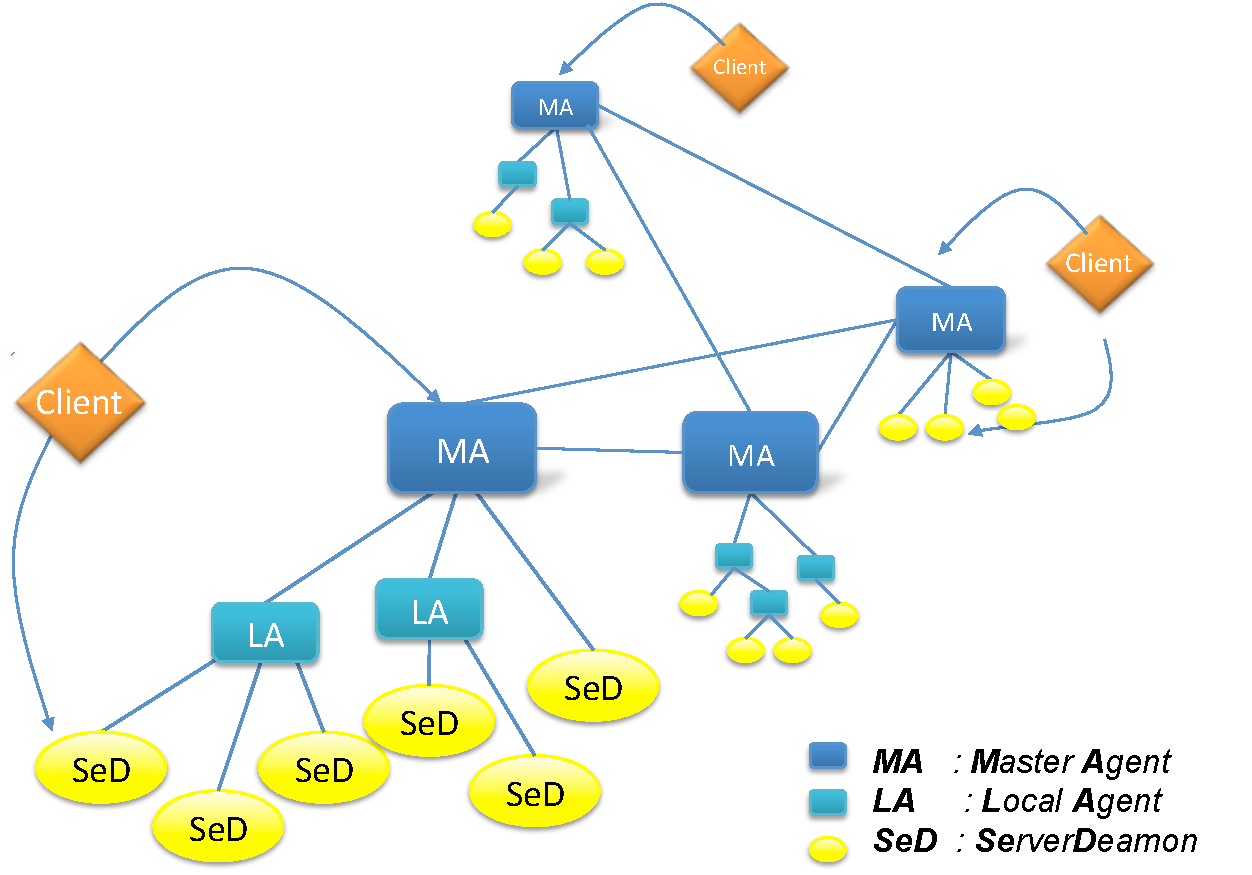
\includegraphics[scale=.7]{fig/global_platform}
  \caption{\label{fig:platform} A hierarchy of \diet agents}
 \end{center}
\end{figure}

%====[ \textsc{Diet} components ]=======================================================
\section{\diet components}
\label{sec:components}

The different components of our software architecture are the
following:

\begin{description}
%....[ Client ]................................................................
\item \textbf{Client}\\ A client is an application which uses \diet to solve
  problems. Many types of clients are able to connect to \diet, from a
  web page, a \pse such as Matlab or \sci, or from a compiled program.
%....[ Master Agent (MA) ].....................................................
\item \textbf{Master Agent (MA)}\\ An MA receives computation requests from
  clients. These requests refer to some \diet problems listed on a reference
  web page. Then the MA collects computation abilities from the servers and
  chooses the best one. The reference of the chosen server is returned to the
  client. A client can be connected to an MA by a specific name server or a web
  page which stores the various MA locations.

%....[ Local Agent (LA) ]......................................................
\item \textbf{Local Agent (LA)}\\ An LA transmits requests and information
  between MAs and servers.  The information stored on an LA is the list of
  services available in the subtree rooted at the LA; for each service, LAs
  store a list of children (agents or servers) that can be contacted to find
  the service. Depending on the underlying network topology, a hierarchy of LAs
  may be deployed between an MA and the servers. Of course, the function of an
  LA is to do a partial scheduling on its subtree, which reduces the workload
  at the MA.

%....[ Server Daemon (SeD) ]...................................................
\item \textbf{Server Daemon (\sed)}\\ A \sed encapsulates a computational
  server. For instance it can be located on the entry point of a parallel
  computer. The information stored on a \sed is a list of the data available
  locally, \ie on the server), the list of problems that can be solved on it,
  and performance-related information such as the amount of available memory or
  the number of resources available. When it registers, a \sed declares the
  problems it can solve to its parent LA or MA.  A \sed can give perfomance and
  hardware information by using the CoRI module or performance predictions for
  some types of problems by using the CoRI module.  Both modules are described
  in Chapter~\ref{chapter:performance}.

\end{description}

%====[ CORBA ]=================================================================
\section{Communications layer}
\label{sec:CORBA}

\nes environments can be implemented using a classic socket communication
layer. Several problems to this approach have been pointed out such as the lack
of portability or limits on the number of sockets that can be opened
concurrently. Our aim is to implement and deploy a distributed \nes environment
that works at a wider scale. Distributed object environments, such as
\emph{Java}, \emph{DCOM} or CORBA have proven to be a good base for building
applications that manage access to distributed services. They not only provide
transparent communications in heterogeneous networks, but they also offer a
framework for the large scale deployment of distributed applications. Being
open and language independent, CORBA was chosen as the communication layer in
\diet.

As recent implementations of CORBA provide communication times close
to that of sockets, CORBA is well suited to support distributed
applications in a large scale Grid environment. New specialized
services can be easily published and existing services can also be
used.  \diet is based upon \emph{OmniORB 4}~\cite{OMNIORB} or later, a
free CORBA implementation that provides good communication
performance.



%====[ \diet INITIALIZATION ]===================================================
\section{\diet initialization}
\label{init}

Figure~\ref{fig:init} shows each step of the initialization of a simple Grid
system. The architecture is built in hierarchical order, each component
connecting to its parent. The MA is the first entity to be started~(1). It
waits for connections from LAs or requests from clients.

\begin{figure}[hbt]
  \begin{center}
    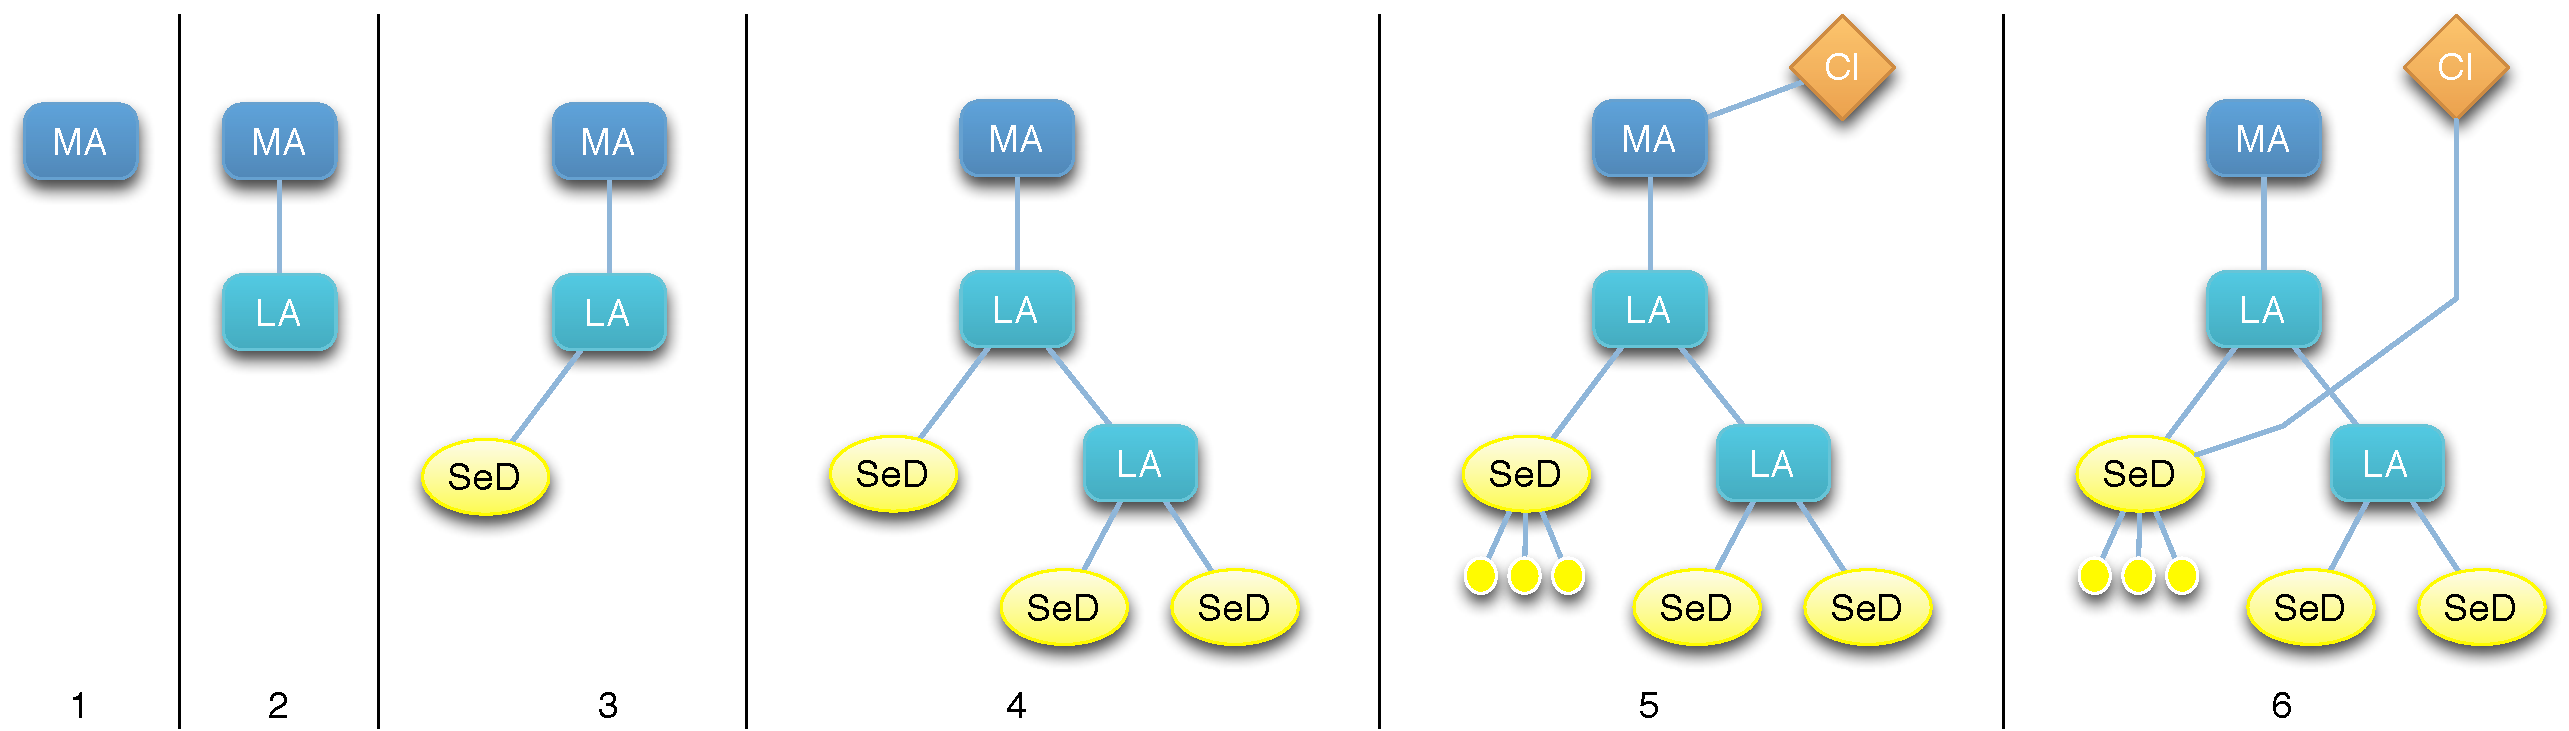
\includegraphics[scale=.35]{fig/init}
    \caption{Initialization of a \diet system.}
    \label{fig:init}
  \end{center}
\end{figure}

In step (2), an LA is launched and registers itself with the MA.  At this step
of system initialization, two kinds of components can connect to the LA: a \sed
~(3), which manages some computational resource, or another LA~(4), to add a
hierarchical level in this branch. When the \sed\ registers to its parent LA,
it submits a list of the services it offers.  The agent then reports the new
service offering through its parent agent until the MA.  If the service was
previously unavailable along that arm of the hierarchy the agents update their
records.  Finally, clients can access the registered service by contacting the
MA~(5) to get a reference to the best server available and then directly
connect to it~(6) to launch the computation.

The architecture of the hierarchy is described in configuration files (see
Section~\ref{sec:diet_config_files}) and each component transmits the local
configuration to its parent. Thus, the system administration can also be
hierarchical. For instance, an MA can manage a domain like a university,
providing prioritary access to users of this domain. Then each laboratory can
run an LA, while each team of the laboratory can run some other LAs to
administrate its own servers. This hierarchical administration of the system
allows local changes in the configuration without interfering with the whole
platform.



%====[ Solving a problem ]=====================================================
\section{Solving a problem}
\label{sec:solvepb}

Assuming that the architecture described in Section~\ref{sec:components}
includes several servers able to solve the same problem, the algorithm
presented below lets an MA select a server for the computation among those
available. This decision is made in four steps.

\begin{itemize}
\item The MA propagates the client request through its subtrees down to the
  capable servers; actually, the agents only forward the request on those
  subtrees offering the service.
\item Each server that can satisfy the request can send his performance and
  hardware information or  an estimation of  the computation time necessary to
  process the request to its ``parent'' (an LA) (via performance prediction
  tools: see Chapter~\ref{chapter:performance}). 
\item Each LA that receives one or more positive responses from its children
  sorts the servers and forwards the best responses to the MA through the
  hierarchy.
\item Once the MA has collected all the responses from its direct children, it
  chooses a pool of ``better'' servers and sends their references to the client.
\end{itemize}

%====[ Extensions ]============================================================
\section{\diet Extensions}
\label{sec:extensions}

%====[ Multi-MA ]==============================================================
\subsection{Multi-MA}
\label{init:multima}

A standard \diet platform gives access to {\sed}s placed under the control of a
MA as explained at the beginning of this chapter. Sometime, it is useful to
connect several MA together. This happens when several organizations wish to
share their resources to offer a larger set of service types and more available
servers. The Multi-MA extension allows this by creating a federation which
shares resources between several MA.

In multi-MA mode, the behavior of a \diet hierarchy does not change when a
client requests a service that is available under the queried MA. However, if a
request sent to a MA does not found a \sed that can resolve its problem, \diet
will forward the request to other MAs of the federation. To read more about
multi-MA, see Chapter~\ref{ch:multiMAextension} and
Chapter~\ref{ch:p2pextension}.

%====[ CoRI ]==============================================================
\subsection{CoRI}
\label{sub:cori}

Collector of Resource Information (CoRI) is a manager for collecting hardware
and performance information.  When \diet is compiled with the appropriate
option, it is possible to get this information via different sub-modules like
 CoRI-Easy. (* if compiled and configured on the \sed machine). See
Chapter~\ref{chapter:performance} for details on using CoRI.

%%%%%%%%%%%%%%%
%% FIXME:
%%  Memory aspects should be treated here.
%%%%%%%%%%%%%%%

%%%%%%%%%%%%%%%
%% FIXME for DIET v1.1
%%%%%%%%%%%%%%%
% In order to solve the problem itself, the client connects to one of
% the servers chosen: it sends its local data and specifies if the
% results should be kept in-place for further computation or if they
% should be brought back. The transfer of persistent operands is
% performed at this stage.
%%%%%%%%%%%%%%%

%%% Local Variables:
%%% mode: latex
%%% ispell-local-dictionary: "american"
%%% mode: flyspell
%%% fill-column: 79
%%% End:
